\documentclass{article}
\usepackage[left=1.9cm,top=2.4cm,right=2.4cm,bottom=2cm]{geometry} 
\usepackage[spanish]{babel}
\usepackage[utf8]{inputenc}
\usepackage{amsmath}
\usepackage{amsfonts}
\usepackage{amssymb}
\usepackage{url}
\usepackage{graphicx}
\usepackage{float}
\usepackage{enumerate} % To use different item symbols in enumerate
\usepackage[inline]{enumitem} % To use different item symbols in enumerate
\usepackage{multicol} % multicolumns
\usepackage{fancyhdr}%Header and Footers
\pagestyle{fancy}
\fancyhf{}
\chead{Universidad Nacional de Colombia\\
Problemas Semestrales}
\cfoot{\thepage}
\renewcommand{\headrulewidth}{0pt} %remove header line
%\renewcommand{\footrulewidth}{1pt} % set footer line

\title{Universidad Nacional de Colombia\\ Fundamentos de Mecánica\\ (PEAMA Sumapaz 2023-I)} %\normalsize{text} normal size of the text font
\author{\textbf{Problemas Semestrales}} %\underline{text} hightlights the text with a line
%\date{\textbf{Nombre: \rule{12cm}{0.15mm}}}

\begin{document}
\maketitle

\subsection*{INDICACIONES}
Las sesiones taller tiene como objetivo evaluar la compresión de diversas tematicas a través la expresión escrita. Por lo tanto, la solución de cada problema debe ser un texto expositivo bien redactado, esto incluye a las ecuaciones y procedimientos matemáticos ya que estos también son texto. Como texto la solución debe tener un propósito claro (calcular,explicar, identificar, describir, relacionar. . . ) ysu redacción debe ser siempre coherente con tal propósito.\\

Teniendo en cuenta lo anterior, los criterios de evaluación de las soluciones son los siguientes:
\begin{enumerate}[label=\roman*)]
\item  \textbf{Descripción de la situación:} Todo problema tiene un contexto o una situación específica. El estudiante debe realizar una descripción de tal contexto y hacer uso de un esquema o figura donde relaciones todos los conceptos, cantidades físicas y/o matemáticas del problema.
\item \textbf{Redacción de la solución:} Todo argumento dado por el estudiante debe ser claro, justificado y debidamente citado o referenciado con la información dada en las clases y/o desde bibliografía relacionada.
\item \textbf{Uso del lenguaje disciplinar y matemático:} Todos los conceptos físicos y matemáticos en la solución deben usarse bien (buen lenguaje y buen manejo de unidades físicas) y las ecuaciones deben ser parte del texto (no una lista de símbolos únicamente).
\item \textbf{Uso de esquemas y figuras:} El estudiante debe hacer buen uso de las imágenes, es decir que debe usar la imagen dentro del texto y todas las variables y/o cantidades que se encuentren en la imagen debe ser definidas en el texto principal.
\end{enumerate}

Las soluciones a los problemas deben ser entregadas de forma \textbf{individual} a lo largo de todo el semestre. 
\section*{PROBLEMAS}
\begin{enumerate}
\item ¿Cuál de los siguientes enunciados es correcto? Justifique su respuesta: \textbf{a)} Es posible que un objeto tenga movimiento en ausencia de fuerzas sobre el objeto. \textbf{b)} Es posible tener fuerzas sobre un objeto en ausencia de movimiento del objeto. \textbf{c)} Ni a) ni b) son correctos. \textbf{d)} Tanto a) como b) son correctos.

\item Es muy que probable que usted haya estado en un elevador que acelera hacia arriba mientras se mueve a pisos superiores. En este caso, se siente más pesado. De hecho, si se para en una báscula en ese momento, la báscula mide una fuerza que tiene una magnitud mayor que su peso. Por lo tanto, tiene evidencia sensorial y medida que lo lleva a creer que es más pesado en esta situación. ¿Es usted más pesado?

\item Una persona pesa un pescado de masa $m$ en una balanza de resorte unida al techo de un elevador, como se ilustra en la figura. Muestre que, si el elevador acelera ya sea hacia arriba o hacia abajo, la balanza de resorte da una lectura que es diferente del peso del pescado.

\begin{figure}[H]
\centering
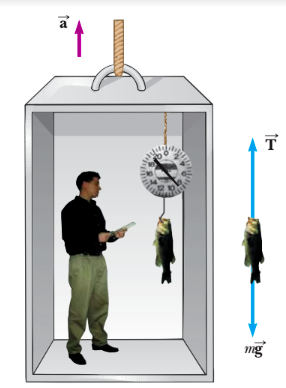
\includegraphics[scale=0.4]{problema_3.png}
\caption{Problema 3.}
\end{figure}

\item Un semáforo que pesa $122$ N (Newtons) cuelga de un cable unido a otros dos cables sostenidos a un soporte como en la figura. Los cables superiores forman ángulos de $37$.$0^{\circ}$ y $53$.$0^{\circ}$ con la horizontal. Estos cables superiores no son tan fuertes como el cable vertical y se romperán si la tensión en ellos supera los
$100$ N. ¿El semáforo permanecerá colgado en esta situación, o alguno de los cables se romperá?

\begin{figure}[H]
\centering
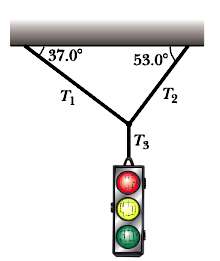
\includegraphics[scale=0.4]{problema_4.png}
\caption{Problema 4.}
\end{figure}

\item Una mujer en un aeropuerto jala su maleta de $20$.$0$ kilogramos (kg) con rapidez constante al jalar de una correa en un ángulo $\theta $ sobre la horizontal (ver figura). Ella jala de la correa con una fuerza de $35$.$0$ N. La fuerza de fricción sobre la maleta es $20$.$0$ N. Dibuje un diagrama de cuerpo libre de la maleta. a) ¿Qué ángulo forma la correa con la horizontal? b) ¿Qué fuerza normal ejerce el suelo sobre la maleta?

\begin{figure}[H]
\centering
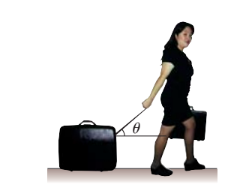
\includegraphics[scale=0.5]{problema_5.png}
\caption{Problema 5.}
\end{figure}

\item Como se muestra en la figura, la base de una máquina de $900$ kg se mueve sobre el piso de concreto mediante una serie de tubos de acero de $100$ milimetros (mm) de diámetro exterior. Si se sabe que el coeficiente de resistencia a la rodadura entre los tubos y la base es de 0.5 mm y entre los tubos y el piso de concreto es de $1$.$25$ mm, determine la magnitud de la fuerza $\textbf{P}$ requerida para mover lentamente la base a lo largo del piso.

\begin{figure}[H]
\centering
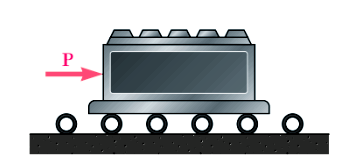
\includegraphics[scale=0.5]{problema_6.png}
\caption{Problema 6.}
\end{figure}

\item Una técnica común aplicada para medir la constante de fuerza de un resorte se demuestra por la configuración de la figura 5. El resorte cuelga verticalmente (figura 5a) y un objeto de masa $m$ se une a su extremo inferior. Bajo la acción de la “carga” $mg$ (siendo $g$ la aceleración gravitacional), el resorte se estira una distancia $d$ desde su posición de equilibrio (figura 5b). Si un resorte se estira $2$.$0$ centímetros (cm) por un objeto suspendido que tiene una masa de $0$.$55$ kg, ¿cuál es la constante de fuerza del resorte?

\begin{figure}[H]
\centering
\begin{tabular}{cc}
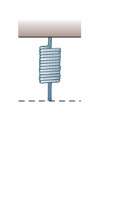
\includegraphics[scale=0.5]{problema_7a.png} & 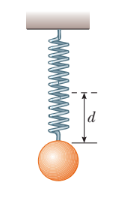
\includegraphics[scale=0.5]{problema_7b.png}\\
(a) & (b)
\end{tabular}

\caption{Problema 7.}
\end{figure}

\textbf{NOTA:} La \textbf{magnitud} de la fuerza $F$ que ejerce un resorte que se comprime o se estira una distancia $\Delta x$ sobre un objeto está dada por $F=-k\Delta x$, donde $k$ es la constante del resorte. 


\item Un hombre quiere cargar un refrigerador en una camioneta con el uso de una rampa a un ángulo $\theta$, como se muestra en la figura. Él afirma que se debe requerir menos trabajo para cargar la camioneta si la longitud $L$ de la rampa aumenta. ¿Esta afirmación es válida?


\begin{figure}[H]
\centering
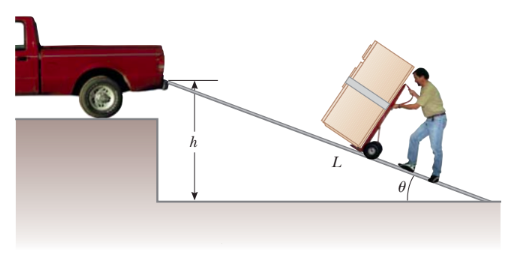
\includegraphics[scale=0.5]{problema_8.png}
\caption{Problema 8.}
\end{figure}


\textbf{NOTA:} El trabajo es la energía transferida a un objeto por la aplicación de una fuerza que lo desplaza una cierta distancia. Cuantitativamente, si $\textbf{F}$ es la magnitud de la fuerza aplicada y $\textbf{d}$ es el vector desplazamiento del objeto, el trabajo $W$ ejercido por la fuerza $\textbf{F}$ está dado por $W=\textbf{F}\cdot\textbf{d}$.

\item Un ascensor tiene una masa de $1600$ kg y transporta pasajeros con una masa combinada de $200$ kg. Una
fuerza de fricción constante de $4000$ N retarda su movimiento. ¿Cuánta potencia debe proporcionar un motor para levantar el elevador y a sus pasajeros con una rapidez constante de $3$.$00$ metros por segundo (m/s)? (\textbf{Pista:} La potencia $P$ se define como la derivada de la energía $E$ respecto al tiempo $t$, $P=dE/dt$. Demuestre que si el ascensor ejerce una fuerza constante $\textbf{F}$, entonces $P=\textbf{F}\cdot \textbf{v}$, donde $\textbf{v}$ la velocidad a la que se mueve el ascensor.)


\item En la figura 7 se muestra un ingenioso dispositivo que explica la conservación de la cantidad de movimiento
y la energía cinética. Consiste de cinco bolas duras idénticas sostenidas por cuerdas de iguales longitudes. Cuando la bola 1 se retira y se libera, después de la colisión casi elástica entre ella y la bola 2, la bola 1 se detiene y la bola 5 se mueve hacia afuera, como se muestra en la figura 7b. Si las bolas 1 y 2 se retiran y liberan, se detienen después de la colisión y las bolas 4 y 5 se balancean hacia afuera, y así por el estilo. ¿Alguna vez es posible que, cuando la bola 1 se libere, se detenga después de la colisión y las bolas 4 y 5 se balanceen en el lado opuesto y viajen con la mitad de la rapidez de la bola 1, como en la figura 7c?

\begin{figure}[H]
\centering
\begin{tabular}{c}
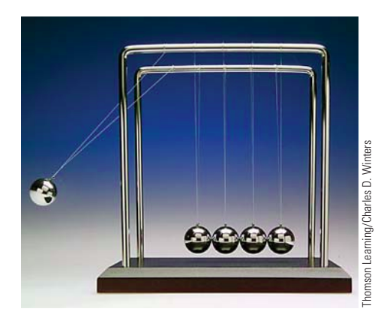
\includegraphics[scale=0.3]{problema_10a.png}\\
(a)\\
\begin{tabular}{cc}
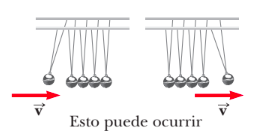
\includegraphics[scale=0.5]{problema_10b.png} & 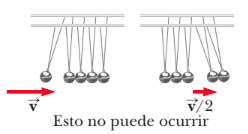
\includegraphics[scale=0.5]{problema_10c.png}\\
(b) & (c)
\end{tabular}
\end{tabular}
\caption{Problema 10.}
\end{figure}

\item Tres objetos de densidad uniforme (una esfera sólida, un cilindro sólido y un cilindro hueco) se colocan en lo alto de un plano inclinado (ver figura). Todos se liberan desde el reposo en la misma elevación y ruedan sin deslizarse. ¿Cuál objeto llega primero a la parte baja? ¿Cuál llega al último? Intente este experimento en casa y observe que el resultado es independiente de las masas y los radios de los objetos. \textbf{Pista:}Consulte el momento de inercia de una esfera, un cilindro sólido y un cilindro hueco. ¿Cuál es la relación entre el momento angular y el momento de inercia?

\begin{figure}[H]
\centering
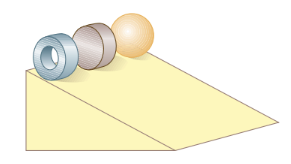
\includegraphics[scale=0.5]{problema_11.png}
\caption{Problema 11.}
\end{figure}

\item La cabeza de una cortadora de pasto tiene $100$ gramos (g) de cuerda devanados en un carrete cilíndrico ligero con diámetro interior de $3$.$00$ cm y diámetro exterior de $18$.$0$ cm, como se muestra en la figura. La cuerda tiene una densidad lineal de $10$.$0$ gramos por metro (g/m). Una sola hebra de la cuerda se extiende $16$.$0$ cm desde el borde exterior del carrete. a) Cuando se enciende, la cortadora aumenta su velocidad de $0$ a $2500$ revoluciones por mininuto (rev/min) en $0$.$215$ segundos (s). ¿Qué potencia promedio entrega el motor de la cortadora a la cabeza mientras acelera?.


\begin{figure}[H]
\centering
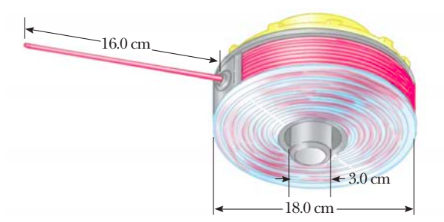
\includegraphics[scale=0.4]{problema_12.png}
\caption{Problema 12.}
\end{figure}

\textbf{Pista:} Demuestre que la potencia $P$ en un movimiento de rotación sobre un eje fijo está dada por $P=\tau\omega$, donde $\tau$ es el torque que ejerce una fuerza para producir el giro y $\omega$ es la rapidez angular del movimieto.


\end{enumerate}

\section{Problemas Conjuntos Algebra Lineal}
\begin{enumerate}


\item La proyección de Mercator es una proyección cartográfica ideada por Gerardus Mercator en 1590 para elaborar mapas de la superficie terrestre. Está proyecció está dada por:

\begin{align*}
x&=R\lambda, \\
y&=R\ln\left|\tan\left(\frac{\pi}{4}+\frac{\phi}{2}\right)\right|,
\end{align*}

donde $R=6371km$ es el radio de la tierra y, $\phi$ y  $\lambda$ son las coordenadas de latitud y longitud de la proyección. Usando está proyección calcule:

\begin{enumerate}
\item Bogotá se encuentrá ubicada aproximadamente entre $3^{\circ}$ y $4^{\circ}$ de latitud, y entre $-73^{\circ}$ y $-74^{\circ}$ de longitud. Determine la distancia $\Delta x=|x(\lambda=-74^{\circ})-x(\lambda=-73^{\circ})|$ y la distancia\\
\noindent $\Delta y=|y(\phi=4^{\circ})-y(\phi=3^{\circ})|$. Compare estas distancias con la extensión de bogotá.
\end{enumerate}

\item La matriz de covarianza $\Sigma$ entre $N$ variables físicas $X_{1},X_{2},\cdots, X_{N}$ se define por:

\begin{align*}
\Sigma(X_{1},X_{2},\cdots, X_{N})&=\left[\begin{matrix}
Var(X_{1}) & Cov(X_{1},X_{2}) & \cdots & Cov(X_{1},X_{N})\\
Cov(X_{2},X_{1}) & Var(X_{2}) & \cdots & Cov(X_{2},X_{N})\\
\vdots & \vdots & \ddots & \vdots \\
Cov(X_{n},X_{1}) & Cov(X_{n},X_{2}) & \cdots & Var(X_{N})
\end{matrix}\right]
\end{align*}

\noindent donde\footnote{En las definiciones de la varianza y covarianza, el simbolo $E(X)$ representa el valor promedio de la variable física $X$.} $Var(X_{i})=E(X_{i}^2)-E(X_{i})^2$ es la varianza de la variable $X_{i}$ y $Cov(X_{i},X_{j})=E(X_{i}\cdot X_{j})-E(X_{i})E(X_{j})$ es la covarianza entre las variables $X_{i}$ y $X_{j}$. Cada variable $X_{i}$ en este contexto corresponde a un conjunto de medidas de variables físicas de algún sistema como lo pueden ser la temperatura del aire, humedad relativa del ambiente, el pH del suelo, entre otros. Teniendo en cuenta está información: 

\begin{enumerate}
\item ¿Qué unidades físicas tiene la varianza y la covarianza entre dos variables? (de ejemplos)
\item ¿Cuál es la interpretación de la varianza y la covarianza entre dos variables?
\item 
\end{enumerate}
asdasda
\end{enumerate}
\end{document}
